\documentclass{article} % For LaTeX2e
\usepackage{times}
\usepackage{hyperref}
\usepackage{url}
\usepackage{times}
\usepackage{tikz}
\usetikzlibrary{arrows,decorations.pathmorphing,fit,positioning}
\usepackage{algorithmic}
\usepackage{mdframed}
\usepackage[margin=1in]{geometry}
\usepackage{amsmath}
%\documentstyle[nips14submit_09,times,art10]{article} % For LaTeX 2.09


\title{Topic extraction for musical genre using lyrical content}


\author{
Sharon Gieske \\
\texttt{00000000}\\
\texttt{email} \\
\and
David van Erkelens\\
\texttt{0000000}\\
\texttt{email} \\
\and
Elise Koster \\
\texttt{5982448}\\
\texttt{koster.elise@gmail.com}
}


% The \author macro works with any number of authors. There are two commands
% used to separate the names and addresses of multiple authors: \And and \AND.
%
% Using \And between authors leaves it to \LaTeX{} to determine where to break
% the lines. Using \AND forces a linebreak at that point. So, if \LaTeX{}
% puts 3 of 4 authors names on the first line, and the last on the second
% line, try using \AND instead of \And before the third author name.

\newcommand{\fix}{\marginpar{FIX}}
\newcommand{\new}{\marginpar{NEW}}

%\nipsfinalcopy % Uncomment for camera-ready version

\begin{document}


\maketitle

\begin{abstract}
Genre classification for music is increasingly important with many online music services around. Manual genre classification is very time-consuming, especially with the large quantities of music available. Thus, a tool that can accurately classify music into a genre would be an economically efficient way to enhance the user experience. This paper proposes an extension of LDA to model topics over genres instead of documents, and proposes that this may improve word-based classifiers.
\end{abstract}

\section{Introduction}

	\subsection{Background}
Music genre classification has been researched mostly using audio signals. While this approach uses the \textit{defining} characteristic of music, namely, its musical structure, an other interesting approach is to use word-based analysis.

\section{Approach}
An extension of LDA is used, which extracts topics over genres instead of documents. A graphical model is supplied in figure \ref{fig:graphical-model}. Derivations can be found in section \ref{ref:derivation}.

\subsection{Derivation}\label{ref:derivation}
\begin{mdframed}
\begin{align}
P(w, z, \varphi, \theta | \alpha, \beta, y) &= P(\varphi | \beta)P(\theta | \alpha)P(z | \theta, y)P(w | \varphi, z)\\
\end{align}
Separate probabilities:
\begin{align}
P(\varphi | \beta) &= \prod\limits_{k=1}^K P(\varphi_k|\beta)\\
P(\theta | \alpha) &= \prod\limits_{g=1}^G P(\theta_g|\alpha)\\
P(z | \theta, y) &= \prod\limits_{i=1}^N \prod\limits_{j=1}^{M_i} P(z_{i,j}|\theta_{y_i})\\
P(w | \varphi, z) &= \prod\limits_{i=1}^N \prod\limits_{j=1}^{M_i} P(w_{i,j}|\varphi_{z_{i,j}})\\
\end{align}
Joined together:
\begin{align}
P(w, z, \varphi, \theta | \alpha, \beta, y) &= \prod\limits_{k=1}^K P(\varphi_k|\beta) \prod\limits_{g=1}^G P(\theta_g|\alpha) \prod^N_{i=1}\prod^{M_i}_{j=1} P(z_{i,j}|\theta_{y_i}) P(w_{i,j}|\varphi_{z_{i,j}})
\end{align}
Integrate over joint:
\begin{align}
\int \int P(w, z, \varphi, \theta | \alpha, \beta, y) d\varphi d\theta &= \int \prod\limits_{k=1}^K P(\varphi_k|\beta) \prod^N_{i=1}\prod^{M_i}_{j=1} P(w_{i,j}|\varphi_{z_{i,j}}) d\varphi\\
&\times \int \prod\limits_{g=1}^G P(\theta_g|\alpha) \prod^N_{i=1}\prod^{M_i}_{j=1} P(z_{i,j}|\theta_{y_i}) d\theta
\end{align}
\subsection{Derivation of $\int \prod\limits_{k=1}^K P(\varphi_k|\beta) \prod^N_{i=1}\prod^{M_i}_{j=1} P(w_{i,j}|\varphi_{z_{i,j}}) d\varphi$}
~\\Use $C(k,w)$ as the number of times word $w$ is assigned to topic $k$ in any document.
\begin{align}
\prod\limits_{k=1}^K P(\varphi_k|\beta) \prod^N_{i=1}\prod^{M_i}_{j=1} P(w_{i,j}|\varphi_{z_{i,j}}) d\varphi
\end{align}
\begin{align}
&= \prod\limits_{k=1}^K \int\frac{\Gamma (\sum\limits_{w=1}^V \beta)}{\prod\limits_{w=1}^V \Gamma(\beta)} \prod\limits_{w=1}^V  \varphi_{k}(w)^{\beta-1}  \prod^N_{i=1}\prod^{M_i}_{j=1} \varphi_{z_{i,j}}(w_{i,j})) d\varphi\\
&= \prod\limits_{k=1}^K \int \frac{\Gamma (V \beta)}{(\Gamma(\beta))^V} \prod\limits_{w=1}^V  \varphi_{k}(w)^{\beta-1}  \prod\limits_{w=1}^V \varphi_{k}(w)^{C(k,w)} d\varphi\\
&= \prod\limits_{k=1}^K \int \frac{\Gamma (V \beta)}{(\Gamma(\beta))^V}  \prod\limits_{w=1}^V \varphi_{k}(w)^{\beta + C(k,w) -1} d\varphi\\
&= \prod\limits_{k=1}^K \frac{\Gamma (V \beta)}{(\Gamma(\beta))^V}  \frac{\prod\limits_{w=1}^V \Gamma(C(k,w)-1)}{\Gamma(\sum\limits_{w=1}^V C(k,w)-1))} \int \frac{\Gamma(\sum\limits_{w=1}^V C(k,w)-1))}{\prod\limits_{w=1}^V \Gamma(C(k,w)-1}  \prod\limits_{w=1}^V \varphi_{k}(w)^{\beta + C(k,w) -1} d\varphi\\
&=  \prod\limits_{k=1}^K \frac{\Gamma (V \beta)}{(\Gamma(\beta))^V}  \frac{\prod\limits_{w=1}^V \Gamma(C(k,w)-1)}{\Gamma(\sum\limits_{w=1}^V C(k,w)-1))}\\
&\propto \prod\limits_{k=1}^K \frac{\prod\limits_{w=1}^V \Gamma(C(k,w)-1)}{\Gamma(\sum\limits_{w=1}^V C(k,w)-1))}
\end{align}
\subsection{Derivation of $\prod\limits_{g=1}^G P(\theta_g|\alpha) \prod^N_{i=1}\prod^{M_i}_{j=1} P(z_{i,j}|\theta_{y_i}) d\theta$}
~\\Use $C(g,k)$ as the number of times topic $k$ is assigned to genre $g$ in any document.
\begin{align}
\prod\limits_{g=1}^G P(\theta_g|\alpha) \prod^N_{i=1}\prod^{M_i}_{j=1} P(z_{i,j}|\theta_{y_i}) d\theta
\end{align}
\begin{align}
&= \prod\limits_{g=1}^G \int\frac{\Gamma (\sum\limits_{k=1}^K \alpha)}{\prod\limits_{k=1}^K \Gamma(\alpha)} \prod\limits_{k=1}^K  \theta_{g}(k)^{\alpha-1}  \prod^N_{i=1}\prod^{M_i}_{j=1} \theta_{y_{i}}(k_{i,j})) d\theta\\
&= \prod\limits_{g=1}^G \int \frac{\Gamma (K \alpha)}{(\Gamma(\alpha))^K} \prod\limits_{k=1}^K  \theta_{g}(k)^{\alpha-1}  \prod\limits_{k=1}^K \theta_g(k)^{C(g,k)} d\theta\\
&= \prod\limits_{g=1}^G \int \frac{\Gamma (K \alpha)}{(\Gamma(\alpha))^K}  \prod\limits_{k=1}^K \varphi_{k}(w)^{\alpha + C(g,k) -1} d\theta\\
&= \prod\limits_{g=1}^G  \frac{\Gamma (K \alpha)}{(\Gamma(\alpha))^K}  \frac{\prod\limits_{k=1}^K \Gamma(C(g,k)-1)}{\Gamma(\sum\limits_{k=1}^K C(g,k)-1))} \int \frac{\Gamma(\sum\limits_{k=1}^K C(g,k)-1))}{\prod\limits_{k=1}^K \Gamma(C(g,k)-1}  \prod\limits_{k=1}^K \varphi_{k}(w)^{\alpha + C(g,k) -1} d\theta\\
&=  \prod\limits_{g=1}^G  \frac{\Gamma (K \alpha)}{(\Gamma(\alpha))^K}  \frac{\prod\limits_{k=1}^K \Gamma(C(g,k)-1)}{\Gamma(\sum\limits_{k=1}^K C(g,k)-1))} \\
&\propto  \prod\limits_{g=1}^G   \frac{\prod\limits_{k=1}^K \Gamma(C(g,k)-1)}{\Gamma(\sum\limits_{k=1}^K C(g,k)-1))} 
\end{align}

\subsection{}
~\\ Use $\neg w_{i,j}$ as collection that not uses word from document i at position j. Use $\widetilde{C}$ as a count that does not include word from document i at position j.
\begin{align}
P(z_{i,j} = k | Z_{\neg w_{i,j}}, \alpha, \beta, W, Y) &\propto \frac{\beta + \widetilde{C}(k, w_{i,j})}{V\beta + \widetilde{C}(k)} \times \frac{\alpha + \widetilde{C}(y_i, k)}{K\alpha + \widetilde{C}(y_i)}
\end{align}
\end{mdframed}

\begin{figure}[htp]
  \centering
  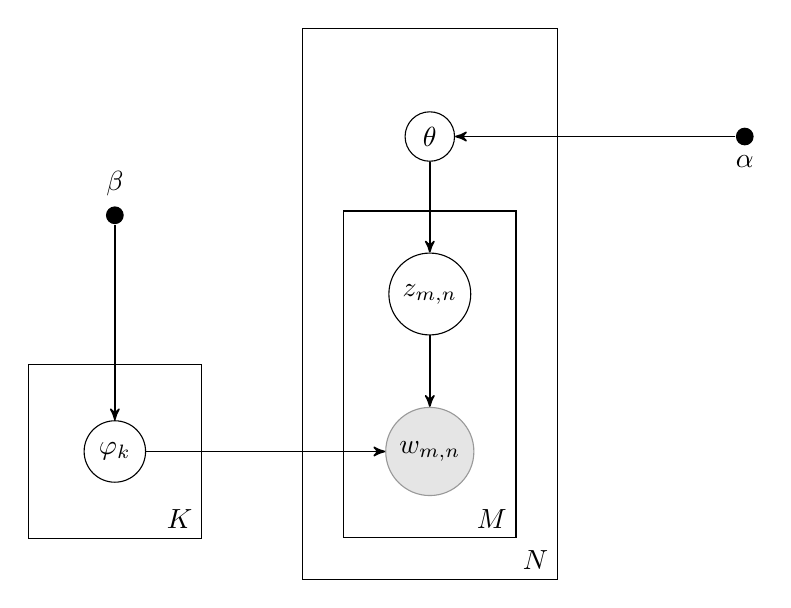
\begin{tikzpicture}
    [
      observed/.style={minimum size=15pt,circle,draw=gray!80,fill=gray!20},
      unobserved/.style={minimum size=15pt,circle,draw},
      hyper/.style={minimum size=1pt,circle,fill=black},
      post/.style={->,>=stealth',semithick},
    ]

    \node (w-j) [observed] at (0,0) {$w_{m,n}$};
    
    \node (z-j) [unobserved] at (0,2) {$z_{m,n}$};

    \node (y) [unobserved] at (0,4) {$\theta$};
    
    \node (w-prior) [unobserved] at (-4,0) {$\varphi_k$};
    
    \node (z-hyper) [label=below:$\alpha$] at (4,4) {};
    
    \filldraw [black] (4,4) circle (3pt);
    
    \node (w-hyper) [label=above:$\beta$] at (-4,3) {};
    
    \filldraw [black] (-4,3) circle (3pt);
    
    \path
    (z-j) edge [post] (w-j)
    
    (z-hyper) edge [post] (y)
    (y) edge [post] (z-j)


    (w-hyper) edge [post] (w-prior)
    
    (w-prior) edge [post] (w-j)
    ;

    \node [draw,fit=(w-j) (y), inner sep=30pt] (plate-context) {};
    \node [above left] at (plate-context.south east) {$N$};
    \node [draw, fit=(w-prior), inner sep=20pt] (plate-prior) {};
    \node [above left] at (plate-prior.south east) {$K$};
    \node [draw,fit=(w-j) (z-j), inner sep=15pt] (plate-token) {};
    \node [above left] at (plate-token.south east) {$M$};

  \end{tikzpicture}
  \caption{Graphical model}
  \label{fig:graphical-model}
\end{figure}

\end{document}
